\documentclass[a4paper]{cas-sc}

\usepackage[numbers]{natbib}
\usepackage{amsmath}
\usepackage{amsfonts}
\usepackage{amssymb}
\usepackage[section]{placeins}

\newcommand{\proglang}[1]{\textit{#1}}
\newcommand{\code}[1]{\texttt{#1}}
\newcommand{\pkg}[1]{\textbf{#1}}

\begin{document}

\let\WriteBookmarks\relax
\def\floatpagepagefraction{1}
\def\textpagefraction{.001}

\shorttitle{\pkg{TCA}: A \proglang{Python} Package for Care Trajectory Clustering}

\shortauthors{Author et al.}

\title[mode=title]{%
  \pkg{TCA} (Trajectory Clustering Analysis): A \proglang{Python} Package for Clustering Unidimensional and Multidimensional Care Trajectories}

\tnotemark[1]
\tnotetext[1]{No external funding was received for this work.}

\author[1]{First Author}%
\cormark[1]
\fnmark[1]
\ead{iauthor@gmail.com}
\credit{Conceptualization, Methodology, Software, Writing – original draft}

\affiliation[1]{%
  organization={Department},
  addressline={Street},
  city={City},
  postcode={100190},
  state={State},
  country={Country}}

\author[2]{Second Author}%
\fnmark[2]
\ead{iiauthor@gmail.com}
\credit{Methodology, Validation, Writing – review \& editing}

\affiliation[2]{%
  organization={Department},
  addressline={Street},
  city={City},
  postcode={10587},
  state={State},
  country={Country}}

\author[1,2]{Third Author}%
\ead{iiiauthor@gmail.com}
\credit{Supervision, Writing – review \& editing}

\cortext[1]{Corresponding author.}

\fntext[1]{These authors contributed equally to this work.}
\fntext[2]{These authors contributed equally to this work.}

\begin{abstract}
\noindent \textbf{Background and Objectives:}
Healthcare trajectory analysis is challenging because healthcare data consist of temporally ordered events that may co-occur across multiple dimensions.
Existing trajectory analysis approaches provide limited support for a unified programmatic analysis of both unidimensional and multidimensional care trajectories in \proglang{Python}.
This study presents \pkg{TCA} (Trajectory Clustering Analysis), an open-source \proglang{Python} package for clustering and analyzing unidimensional and multidimensional care trajectories.

\textbf{Methods:}
For unidimensional trajectories, \pkg{TCA} implements six dissimilarity measures combined with three clustering algorithms.
For multidimensional trajectories, \pkg{TCA} integrates SWoTTeD (Sliding Window for Temporal Tensor Decomposition), which represents trajectories as a three-dimensional tensor and extracts temporal phenotypes through penalized tensor decomposition.

\textbf{Results:}
\pkg{TCA} was evaluated on three datasets: a unidimensional clinical sequence dataset comprising 1,317 patients over 18 months; a multidimensional synthetic cohort generated using Synthea, comprising 901 patients, 10 medications, and 179 days; and real-world oncological care trajectories from the VICAN5 cohort, comprising 1,336 patients with colorectal cancer, four treatment types, and 24 months.
In the unidimensional setting, \pkg{TCA} identified clinically interpretable clusters with distinct care progression profiles.
In the multidimensional setting, SWoTTeD extracted temporal phenotypes and supported hyperparameter tuning for tensor decomposition.

\textbf{Conclusions:}
\pkg{TCA} provides an open-source \proglang{Python} framework for the analysis of unidimensional and multidimensional care trajectories.
By integrating trajectory clustering and temporal tensor decomposition within a single package, \pkg{TCA} facilitates the application of advanced trajectory analysis methods in biomedical research.
The package is available at \url{https://github.com/QuanTIMLab/TrajectoryClusteringAnalysis}.
\end{abstract}

\begin{highlights}
\item Unified \proglang{Python} framework for care trajectory clustering.
\item Six dissimilarity measures and three clustering algorithms are available.
\item Temporal phenotypes are extracted using tensor decomposition.
\item Hyperparameters can be tuned for temporal tensor decomposition.
\item Evaluated on clinical, synthetic, and cancer care trajectories.
\end{highlights}

\begin{keywords}
  trajectory clustering \sep
  care trajectories \sep
  sequence analysis \sep
  tensor decomposition \sep
  phenotyping \sep
  Python \sep
\end{keywords}

\maketitle

\section{Background and Objectives}\label{sec:background}

Understanding how patients progress over time, including which treatments they receive, in what order, and at what pace, can support the identification of care profiles and inform the organisation of healthcare services.
Large-scale medico-administrative databases and electronic health records enable such trajectories to be studied at the population level, but analysis remains difficult because temporal ordering, event durations, and co-occurring clinical events must be considered simultaneously.
 
Care trajectories can be classified as \emph{unidimensional}, in which a single clinical state is observed at each time point $t$ (e.g., under treatment or recovered, but not both), or \emph{multidimensional}, in which multiple events may co-occur at the same time point (e.g., several treatments in the same month). 
Multidimensional trajectories provide a more comprehensive representation of patient care but are harder to analyze with classical sequence analysis methods.
 
Unidimensional trajectories are commonly analyzed by computing pairwise dissimilarities followed by clustering~\cite{denteuling2026clustering,pacca2025sequence}, using measures provided by the \proglang{R} package \pkg{TraMineR}~\cite{traminer}. 
For multidimensional trajectories, SWoTTeD (\emph{Sliding Window for Temporal Tensor Decomposition})~\cite{sebia2024swotted} represents trajectories as a three-dimensional tensor and applies tensor decomposition to extract temporal phenotypes, i.e., recurrent patterns of co-occurring events across sliding time windows.
 
Available software solutions, however, remain fragmented: \pkg{TraMineR} primarily supports unidimensional sequence analysis, whereas multidimensional analysis requires separate implementations, limiting accessibility for health data professionals without programming expertise.
To address this gap, we developed \pkg{TCA} (\emph{Trajectory Clustering Analysis}), an open-source \proglang{Python} package providing a unified framework integrating trajectory clustering and temporal tensor decomposition for unidimensional and multidimensional care trajectory analysis.

\section{Methods}\label{sec:implementation}

\pkg{TCA} is implemented in \proglang{Python} and freely available on PyPI and GitHub. 
The package handles both unidimensional and multidimensional data through a \code{mode} parameter, letting users switch analysis modes without changing their core workflow. 
For unidimensional analysis, the workflow chains data preparation, pairwise distance computation, and clustering. 
For multidimensional analysis, the pipeline first builds and decomposes the data tensor via SWoTTeD to extract temporal phenotypes and patient-specific activation matrices, then clusters patients on these phenotype profiles.

\textbf{AI assistance:} Large language model (LLM) assistance was used during the development of \pkg{TCA} for code optimisation purposes.
All code was reviewed, tested, and validated by the authors, who take full responsibility for the accuracy and integrity of the final implementation.

\subsection{Unidimensional analysis}\label{sec:uni}

Unidimensional analysis consists of three main steps: data preparation, dissimilarity matrix computation, and clustering.
For patient $k \in \{1,\ldots,K\}$, a clinical trajectory is represented as a sequence
$\boldsymbol{x}_k = (x_{k,1}, \ldots, x_{k,T})$, where $K$ is the number of patients, $T$ is the observation duration, and $x_{k,t}$ denotes the clinical state observed at time $t \in \{1,\ldots,T\}$.

\textbf{Data preparation.}
The \pkg{TCA} model is instantiated in \code{'unidimensional'} mode by specifying the patient identifier column, the alphabet of clinical states, and their display labels. 
The package expects data in wide format (one row per patient, one column per time point); data provided in long format must first be reshaped.

\textbf{Substitution cost matrix.}
Before computing sequence dissimilarities, a substitution cost matrix encoding the dissimilarity between pairs of clinical states can be defined through the \code{compute\_substitution\_cost\_matrix} function, using one of three methods: 
\emph{constant} (equal cost for all substitutions, suitable when no prior information is available), 
\emph{frequency-based} (costs derived from observed transition frequencies, with lower costs for states that frequently follow one another), 
or \emph{custom} (user-specified costs for individual state pairs, incorporating domain-specific knowledge).

\textbf{Dissimilarity measures.}
Because no single measure is universally appropriate for healthcare trajectories, \pkg{TCA} provides several complementary measures that capture different aspects of temporal similarity through the \code{compute\_distance\_matrix} function.
\begin{itemize}
  \item \emph{Euclidean}: numerical-vector representation, applicable only to equal-length sequences.
  \item \emph{Hamming}: proportion of differing positions between equal-length sequences, optionally weighted by a substitution cost matrix.
  \item \emph{Levenshtein} \citep{levenshtein1966binary}: minimum number of edit operations to transform one sequence into another, accommodating sequences of different lengths.
  \item \emph{Optimal Matching} (OM) \citep{andjohn1986optimal}: incorporates substitution and insertion/deletion costs, widely used in care trajectory analysis.
  \item \emph{Dynamic Time Warping} (DTW): elastic temporal alignment, usable with a standard or custom metric.
  \item \emph{Global Alignment Kernel} (GAK) \citep{denteuling2026clustering}: kernel-based similarity based on global alignment principles.
\end{itemize}

\textbf{Clustering.}
Once the dissimilarity matrix $d(\boldsymbol{x}_k,\boldsymbol{x}_{k'})$ has been computed, three clustering approaches are available: 
hierarchical agglomerative clustering (HAC, via \code{hierarchical\_clustering}, supporting several linkage criteria including Ward's method and single linkage); 
$k$-medoids \citep{denteuling2026clustering} (via \code{kmedoids\_clustering}, using the \code{fasterpam} algorithm, with each cluster represented by its medoid trajectory); 
and $k$-means, available in two variants : \code{kmeans\_on\_wide\_format}, operating on numerically encoded sequences $\boldsymbol{x}_k$ in wide format (retaining temporal positions), 
and \code{kmeans\_on\_frequency}, operating on patient-level state-frequency vectors irrespective of temporal order.

\textbf{Visualization.}
\pkg{TCA} provides visualization functions to facilitate interpretation of clustering results, including heatmaps of individual trajectories ordered by cluster and summary plots of clinical-state distribution within each cluster.

\subsection{Multidimensional analysis (SWoTTeD)}\label{sec:multi}

\textbf{Data preparation.}
The \pkg{TCA} class is instantiated in \code{'multidimensional'} mode by specifying the patient identifier, time, and event columns. 
For each patient $k$, the trajectory $\boldsymbol{x}_k$ is represented as a binary matrix of size $n \times T_k$ ($n$: number of event types, $T_k$: observation duration), with entry $(i,j)=1$ if event $i$ occurs at time $j$ and $0$ otherwise. 
The matrices of all patients are stacked to form a three-dimensional tensor $\mathcal{X}$. 
The package expects data in long format (one row per patient-event-time combination) and converts them into this binary tensor representation.

\textbf{Temporal phenotypes and activation matrices.}
The core idea of SWoTTeD~\cite{sebia2024swotted} is to decompose the trajectory data into a set of temporal phenotypes shared across patients and patient-specific activation matrices describing when and with what intensity each phenotype occurs.
Given $R \in \mathbb{N}^*$ phenotypes of duration $\omega \in \mathbb{N}^*$, the model estimates:
\begin{itemize}
  \item $\mathcal{P} \in \mathbb{R}_+^{R \times n \times \omega}$, a tensor containing $R$ temporal phenotypes, each represented by a matrix of size $n \times \omega$;
  \item $\mathcal{W} = \left\{W^{(k)} \in \mathbb{R}_+^{R \times (T_k-\omega+1)}\right\}_{k \in [K]}$, a set of patient-specific activation matrices, where a non-zero entry at $(r,t)$ indicates the activation of phenotype $r$ at time $t$ for patient $k$.
\end{itemize}
 
The reconstruction of patient $k$'s trajectory is defined using a convolution operator $\circledast$:
\begin{equation}
  X^{(k)} \approx \widehat{X}^{(k)} = \mathcal{P} \circledast W^{(k)}
  \label{eq:x_eq}
\end{equation}
 
Because multiple phenotypes may be activated simultaneously, the model can represent co-occurring clinical events and overlapping temporal patterns.

\textbf{Optimization and regularization.}
The model is trained by minimizing a penalized loss, whose reconstruction term $\mathcal{L}^{SW}$ follows the Bernoulli-based formulation of SWoTTeD:
\begin{equation}
  \mathcal{L}^{SW} = \arg\min_{\mathcal{W},\,\mathcal{P}} \sum_{k=1}^{K} \sum_{t=1}^{T_k} \sum_{i=1}^{n} \log\!\left(\hat{x}^{(k)}_{i,t}+1\right) -x^{(k)}_{i,t}\log\!\left(\hat{x}^{(k)}_{i,t}\right)
  \label{eq:recon_loss}
\end{equation}
subject to $\mathcal{W}\geq0$ and $\mathcal{P}\geq0$.
 
The total loss $\ell$ extends the reconstruction term with two regularization penalties:
\begin{equation}
  \ell = \mathcal{L}^{SW} + \alpha\|\mathcal{P}\|_1 + \gamma\sum_{k=1}^{K}S\!\left(\boldsymbol{W}^{(k)}\right)
  \label{eq:loss}
\end{equation}
 
The sparsity term $\alpha\|\mathcal{P}\|_1$ penalizes dense phenotypes, encouraging patterns with a limited number of active events and thereby improving interpretability. 
The non-succession term $\gamma\sum_{k=1}^{K}S(\boldsymbol{W}^{(k)})$ penalizes repeated activations of the same phenotype within overlapping windows, defined as:
\begin{equation}
  S\!\left(\boldsymbol{W}^{(k)}\right) = \sum_{r=1}^{R}\sum_{t=1}^{T_k} w_{r,t} \log\!\left( \sum_{\tau=t-\omega}^{t+\omega}w_{r,\tau}
  \right)
  \label{eq:non_succession}
\end{equation}
 
This discourages representing repeated events as multiple overlapping activations of the same phenotype. 
$\alpha$ and $\gamma$ are user-specified hyperparameters controlling the relative contribution of the two terms. 
Optimization uses Adam within a \proglang{PyTorch Lightning} training loop, with a \emph{ReduceLROnPlateau} learning-rate scheduler.

\textbf{Regularization term normalization.}
To make the regularization weights comparable across datasets, the dimensionless relative weights $\tilde{\alpha}$ and $\tilde{\gamma}$ are converted into absolute weights as follows:
\begin{equation}
  \alpha = \tilde{\alpha}\cdot \frac{K\cdot T\cdot n}{R\cdot n\cdot\omega},
  \qquad
  \gamma = \tilde{\gamma}\cdot \frac{K\cdot T\cdot n}{R\cdot T\cdot K}
  \label{eq:normalized_reg}
\end{equation}
where $K$, $T$, $n$, $R$, and $\omega$ denote, respectively, the number of patients, maximum observation duration, number of event types, number of phenotypes, and phenotype window length.

\textbf{Patient clustering.}
After decomposition, each patient's activation matrix $W^{(k)}$ is summarized as an $R$-dimensional normalized intensity vector (activation intensity per phenotype, normalized by observation duration), on which clustering is then performed.

\textbf{Evaluation metrics.}
Two metrics assess decomposition quality. The \emph{FIT} metric~\cite{sebia2024swotted,Afshar2018} measures reconstruction quality:
\begin{equation}
  \mathrm{FIT}_X = 1- \frac{\sum_{k=1}^{K} \left\|X^{(k)}-\widehat{X}^{(k)}\right\|_F} {\sum_{k=1}^{K}\left\|X^{(k)}\right\|_F}
  \label{eq:fit}
\end{equation}
where $\|\cdot\|_F$ denotes the Frobenius norm; values closer to 1 indicate better reconstruction. During training, $\mathrm{FIT}_X$ was evaluated every 10 epochs, with early stopping applied when the metric failed to improve by at least $\delta=10^{-4}$ over 10 consecutive evaluations, after which the model was restored to the best checkpoint.
 
The \emph{phenotype diversity} metric~\cite{sebia2024swotted} quantifies redundancy among the $R$ extracted phenotypes. Each phenotype $\mathcal{P}_r$ is normalized as:
\begin{equation}
  \tilde{p}_r = \frac{\mathrm{vec}(\mathcal{P}_r)} {\|\mathrm{vec}(\mathcal{P}_r)\|_2}
  \label{eq:normalisation}
\end{equation}
and the global diversity is defined as the mean pairwise cosine distance:
\begin{equation}
  \mathrm{div}(\mathcal{P}) = \binom{R}{2}^{-1} \sum_{1\leq i<j\leq R} \left(1-\langle\tilde{p}_i,\tilde{p}_j\rangle\right)
  \label{eq:div_globale}
\end{equation}
Values close to 0 indicate highly similar phenotypes, whereas values close to 1 indicate more distinct event combinations.
 
In practice, $\mathrm{FIT}_X$ and $\mathrm{div}(\mathcal{P})$ may be in tension: configurations with higher reconstruction quality can produce more redundant phenotypes, and vice versa. 
Hyperparameter tuning therefore considers $R$, $\omega$, $\tilde{\alpha}$, and $\tilde{\gamma}$ jointly to identify a suitable balance.

\section{Results}\label{sec:results}

\subsection{Unidimensional results}\label{sec:uni_res}

The unidimensional analysis was conducted on the \code{unidimensional\_data} dataset~\citep{larmarange_analyseR}, which initially contains 2 929 patients followed over 50 months. 
We restrict the analysis to the first 18 months, retaining only patients with complete observations over this period so that all sequences are fully observed and of equal length, resulting in 1 317 patients. 
At each month $t$, each patient is assigned one of four clinical states, representing successive stages of a care pathway from diagnosis to viral suppression: 
\begin{itemize}
  \item \textbf{D} (\textit{Diagnosed}, not yet in care),
  \item \textbf{C} (\textit{In care}, not yet on treatment),
  \item \textbf{T} (\textit{Under treatment}, infection not yet controlled),
  \item \textbf{S} (\textit{Controlled}, infection successfully suppressed).
\end{itemize}

 
Each patient is also characterised by sociodemographic and geographic covariates, not used for clustering but used for interpreting the resulting clusters: 
\begin{itemize}
  \item \textbf{sex} (male/female), 
  \item \textbf{age} group (young/adult/senior), 
  \item \textbf{education} level (primary/secondary/higher), 
  \item \textbf{wealth} index (poor/moderate/rich), 
  \item \textbf{distance\_clinic}, geographic proximity to the nearest healthcare center (close/far).
\end{itemize}

\textbf{Distance computation.}
Optimal Matching (OM) was selected as the primary dissimilarity measure, being particularly suited to clinical state sequences where both the nature and timing of transitions matter~\cite{andjohn1986optimal}. 
A custom substitution cost matrix was defined via \code{compute\_substitution\_cost\_matrix}, assigning higher costs to clinically less plausible transitions (e.g., moving directly from \textit{D} to \textit{S}); the indel cost is set by \pkg{TCA} to half the maximum substitution cost by default, but can also be specified manually. 
Table~\ref{tab:runtimes} reports the runtimes and theoretical complexities of all available distance metrics on this dataset.
 
\begin{table}[h]
\centering
\caption{Theoretical complexity and runtime  of distance metrics available in \pkg{TCA}, measured on the unidimensional dataset (1 317 patients, 18 time points).}
\label{tab:runtimes}
\begin{tabular}{lcc}
\hline
\textbf{Metric} & \textbf{Complexity} & \textbf{Runtime} \\
\hline
Optimal Matching & $\mathcal{O}(K^2 T^2)$ & $3$~s \\
Hamming & $\mathcal{O}(K^2 T)$ &  $0,1$~s  \\
Levenshtein & $\mathcal{O}(K^2 T^2)$ & $17$~s \\
DTW & $\mathcal{O}(K^2 T^2)$ & $216$~s \\
GAK & $\mathcal{O}(K^2 T^2)$ & $375$~s \\
\hline
\end{tabular}
\end{table}

\textbf{Clustering.}
Hierarchical agglomerative clustering (HAC) with Ward's linkage was applied to the OM distance matrix. The dendrogram (Figure~\ref{fig:dendrogram}) reveals a clear four-group structure, confirmed by the elbow method on the within-cluster inertia curve, and HAC ($k=4$) was retained.
 
The four clusters (Figure~\ref{fig:heatmap_cah}) are interpreted as follows:
 
\begin{itemize}
    \item \textbf{Incomplete} ($n = 125$): patients who enter care but do not initiate or sustain treatment over the observation period.
    \item \textbf{Out of care} ($n = 577$): patients who remain predominantly in the diagnosed state throughout, without entering or maintaining engagement in care.
    \item \textbf{Slow} ($n = 268$): patients who progress through care but at a slower pace, reaching controlled infection only after month~6.
    \item \textbf{Fast} ($n = 347$): patients who rapidly transition through the care cascade and reach controlled infection within the first months.
\end{itemize}
 
\pkg{TCA} provides visualization functions to support cluster interpretation, including sequence heatmaps, state distribution plots, and sociodemographic breakdowns.

\begin{figure}[htbp]
  \centering
  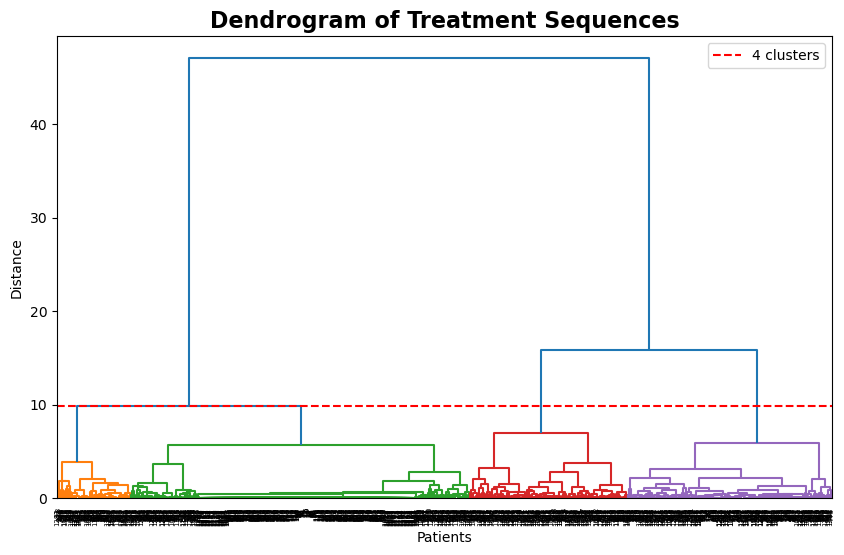
\includegraphics[width=\columnwidth]{dendrogramme_OM}
  \caption{Dendrogram of treatment sequences obtained by hierarchical agglomerative clustering (Ward's linkage) on the Optimal Matching distance matrix (1 317 patients, 18 months).}
  \label{fig:dendrogram}
\end{figure}

\begin{figure}[htbp]
  \centering
  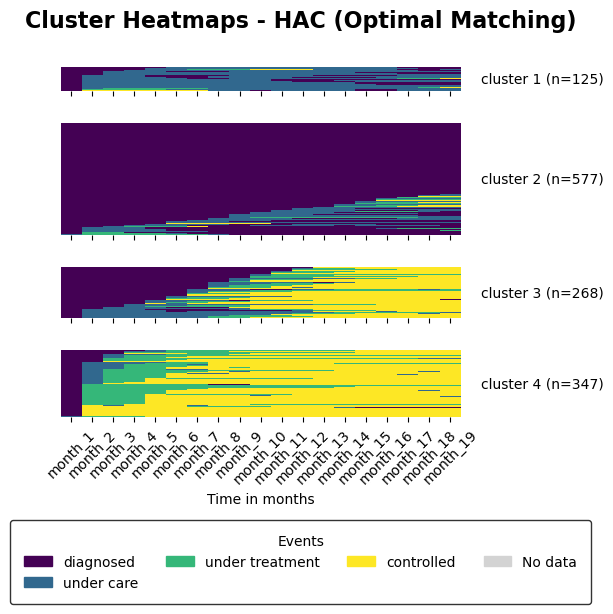
\includegraphics[width=\columnwidth]{cah_OM}
  \caption{Heatmaps of individual trajectories by cluster, obtained by hierarchical agglomerative clustering ($k = 4$) on the Optimal Matching distance matrix.}
  \label{fig:heatmap_cah}
\end{figure}

\FloatBarrier

\subsection{Multidimensional results}\label{sec:multi_res}

The multidimensional analysis was first conducted on a synthetic dataset generated via Synthea \citep{walonoski2020synthea}, comprising 901 patients with chronic conditions followed over 179 days, with event types corresponding to ten medications covering cardiovascular, respiratory, and metabolic treatments (Albuterol and Fluticasone inhalers, Insulin, Metformin, Hydrochlorothiazide, Amlodipine, Atenolol, Nitroglycerin, Simvastatin). 
This controlled setting, with daily granularity, a large number of event types, and a long observation period, provides a suitable starting point for validating the hyperparameter tuning workflow before applying it to real-world data.
 
The analysis was then extended to real-world oncological care trajectories from the VICAN5 survey (VIe 5 ans après le CANcer, a French national cohort of cancer survivors~\cite{Bouhnike005971}), comprising 1 336 patients with colorectal cancer followed over 24 months at monthly granularity, with only four event types (intravenous chemotherapy, oral chemotherapy, surgery, radiotherapy). 
The larger, sparser, more heterogeneous cohort tests whether conclusions from the synthetic setting generalize to a realistic context.
 
In both cases, the goal is to extract $R$ temporal phenotypes jointly achieving $\text{FIT}_X$ close to 1 (accurate reconstruction) and $\text{div}(\mathcal{P})$ close to 1 (distinct, complementary phenotypes). 
These objectives are often in tension: configurations maximizing $\text{FIT}_X$ tend to produce redundant phenotypes, and vice versa. 
Hyperparameter tuning therefore aims to balance them by guiding the selection of $R$, $\omega$, $\tilde{\alpha}$, and $\tilde{\gamma}$.

\subsubsection{Synthea synthetic cohort}\label{sec:synthea_res}

\textbf{Experimental setup.}
The tensor constructed from the Synthea dataset has dimensions $K = 901$ patients, $n = 10$ event types, and a maximum duration of $T = 179$ days. 
Each SWoTTeD trial runs for up to 500 epochs with early stopping (patience of 5 evaluations, monitored on $\text{FIT}_X$), a learning rate of $10^{-2}$, and a \emph{ReduceLROnPlateau} scheduler (factor 0.5, patience 10).

\textbf{Hyperparameter search.}
Ten configurations were sampled with \texttt{random.seed(42)} from the following space (both regularisation weights on a log scale): rank $R \in \{2, \ldots, 5\}$, window length $\omega \in \{2, \ldots, 10\}$ days, normalised sparsity weight $\tilde{\alpha} \in [10^{-5},\, 2 \times 10^{-4}]$, normalised non-succession weight $\tilde{\gamma} \in [0.1,\, 2.0]$. 
The rank bound avoids empty or redundant phenotypes given dataset sparsity; the window range was reduced after observing that only the first few days of longer windows were consistently activated. 
The search required approximately 1 360 minutes.
 
Configurations were ranked by descending $\text{FIT}_X$ then $\text{div}(\mathcal{P})$ (Table~\ref{tab:results_synthea}), but these served only as ranking criteria: phenotypes were also visually inspected, since a configuration can achieve high scores on both metrics while containing near-inactive phenotypes, in which case diversity stays high despite limited interpretable information. 
The final configuration was selected jointly on quantitative metrics and interpretability.

\begin{table}[htbp]
\centering
\caption{Random search results on the Synthea cohort, sorted by descending $\text{FIT}_X$ then descending $\text{div}(\mathcal{P})$.}
\label{tab:results_synthea}
\begin{tabular}{ccccccc}
\toprule
$R$ & $\omega$ & $\tilde{\alpha}$ & $\tilde{\gamma}$ & best $\text{FIT}_X$ & $\text{div}(\mathcal{P})$ & Time \\
\midrule
3 & 5 & $1.90$ & $0.91$ & $0.576$ & $0.972$ & $7 624$~s \\
2 & 2 & $3.74$ & $1.04$ & $0.572$ & $1.0$ & $7 873$~s \\
2 & 8 & $0.11$ & $0.66$ & $0.547$ & $0.999$ & $8 775$~s \\
5 & 3 & $0.57$ & $2.40$ & $0.535$ & $0.995$ & $9 000$~s \\
3 & 3 & $1.37$ & $4.83$ & $0.527$ & $0.957$ & $9 866$~s \\
5 & 5 & $0.25$ & $0.46$ & $0.461$ & $0.90$ & $8 842$~s \\
4 & 2 & $1.80$ & $1.25$ & $0.419$ & $0.854$ & $8 699$~s \\
2 & 8 & $0.14$ & $6.33$ & $0.414$ & $0.459$ & $8 993$~s \\
2 & 4 & $1.64$ & $1.39$ & $0.365$ & $0.879$ & $8 549$~s \\
3 & 10 & $0.33$ & $1.79$ & $0.038$ & $0.361$ & $3 413$~s \\
\bottomrule
\end{tabular}
\end{table}

\textbf{Results.}
The best configuration corresponds to $R = 3$, $\omega = 5$ days, $\tilde{\alpha} = 1.76 \times 10^{-4}$ and $\tilde{\gamma} = 2.74 \times 10^{-1}$ ($\alpha = 1.90$, $\gamma = 9.14 \times 10^{-1}$), yielding $\text{FIT}_X = 0.576$ and $\text{div}(\mathcal{P}) = 0.972$. 
Training ran for 150 epochs before early stopping (Figure~\ref{fig:training_synthea}): $\text{FIT}_X$ increases from 0.05 at epoch~10 to a peak of 0.576 around epoch~100, then declines as the non-succession term gains weight, accounting for approximately 28\% of the final loss versus a marginal 3\% for the sparsity term, indicating the model is primarily constrained by the temporal succession penalty.
 
The three discovered phenotypes (Figure~\ref{fig:phenos_synthea}) capture distinct medication profiles: 
\begin{itemize}
  \item \textbf{Phenotype~1} shows a faint signal on Atenolol Combo and Fluticasone Inhaler (near-inactive/background profile); 
  \item \textbf{Phenotype~2} shows strong, concentrated activation of Albuterol and Fluticasone Inhaler over the $\omega = 5$-day window (respiratory treatment pattern); 
  \item \textbf{Phenotype~3} shows moderate activation of cardiovascular/metabolic medications (HCTZ~25mg, Insulin, Metformin : chronic disease management profile).
\end{itemize}

Reconstruction quality varies with medication profile. 
For patient~18, dominated by Albuterol and Fluticasone Inhaler (Phenotype~2), reconstruction is very faithful, correctly recovering timing and identity of episodes (Figure~\ref{fig:rec18_synthea}). 
For patient~21 (Atenolol Combo, Metformin, Insulin, HCTZ~25mg), reconstruction is less precise, capturing the general structure but attenuating or misplacing some events, reflecting the difficulty of reconstructing complex polypharmacy with only three phenotypes (Figure~\ref{fig:rec21_synthea}). 
This matches cohort composition: 586/901 patients (65.0\%) received both respiratory medications, making that pattern dominant, whereas polypharmacy profiles (at most 19.4\% for Metformin) form a smaller subgroup, explaining Phenotype~3's lower fidelity.

\textbf{Clustering.}
A pairwise Euclidean distance matrix on the normalised phenotype intensity vectors, followed by HAC (Ward linkage), revealed a clear three-cluster structure (Figure~\ref{fig:dendro_synthea}) with $n_1 = 508$, $n_2 = 304$, and $n_3 = 89$ patients (Figure~\ref{fig:heatmap_synthea}): 
\begin{itemize}
  \item Cluster~1 is dominated by Phenotype~2 (respiratory medications, Albuterol/Fluticasone), Phenotypes~1 and~3 largely absent; 
  \item Cluster~2 shows moderate, heterogeneous activation of Phenotypes~2 and~3 (patients combining respiratory and chronic disease medications);
  \item Cluster~3 shows strong Phenotype~1 and moderate Phenotype~3, Phenotype~2 essentially absent (cardiovascular/metabolic medications without significant respiratory treatment).
\end{itemize}

\begin{figure}[htbp]
    \centering
    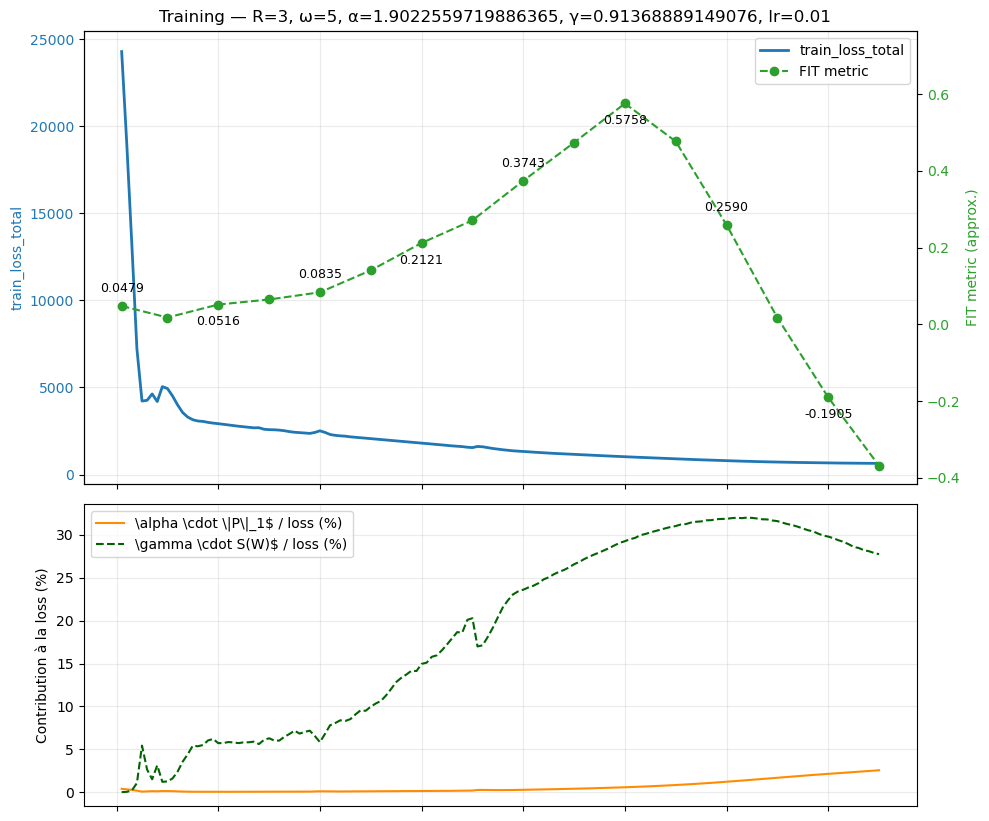
\includegraphics[width=\textwidth]{training_SYNTHEA.png}
    \caption{Training history of the retained SWoTTeD configuration on the Synthea cohort ($R=3$, $\omega=5$, $\alpha=1.90$, $\gamma=9.14\times10^{-1}$, $\text{lr}=10^{-2}$). 
    \textit{Top}: total training loss (blue) and approximate $\text{FIT}_X$ metric (green dashed) over 150 epochs.
    \textit{Bottom}: relative contributions of the sparsity term $\alpha\cdot\|\mathcal{P}\|_1$ (orange) and the non-succession term $\gamma\cdot S(\mathcal{W})$ (green dashed) to the total loss.}
    \label{fig:training_synthea}
\end{figure}

\begin{figure}[htbp]
    \centering
    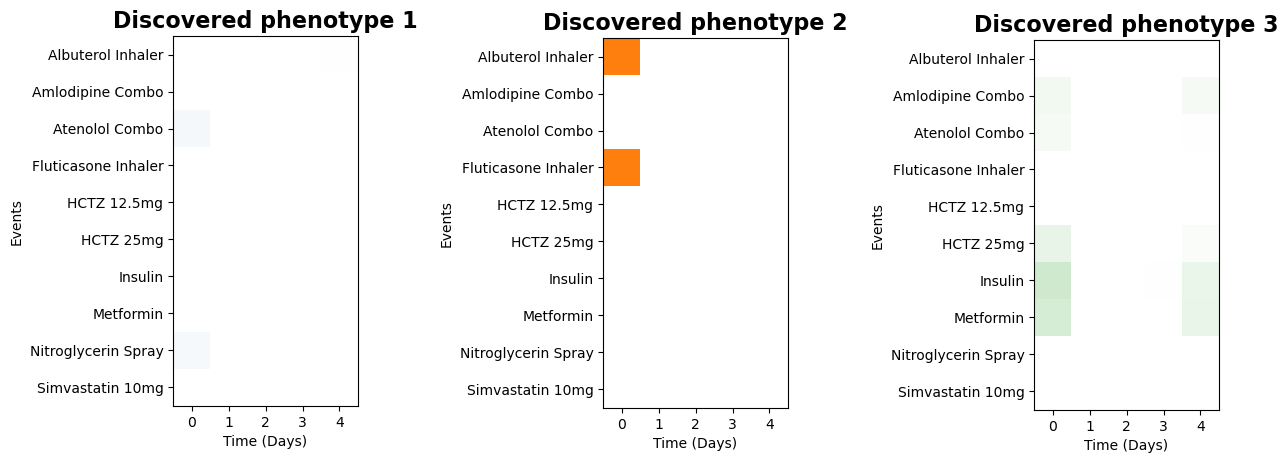
\includegraphics[width=\textwidth]{phenos_SYNTHEA.png}
    \caption{The three phenotypes discovered by SWoTTeD on the Synthea cohort ($R=3$, $\omega=5$, $\alpha=1.90$, $\gamma=9.14\times10^{-1}$, $\text{lr}=10^{-2}$).}
    \label{fig:phenos_synthea}
\end{figure}

\begin{figure}[htbp]
    \centering
    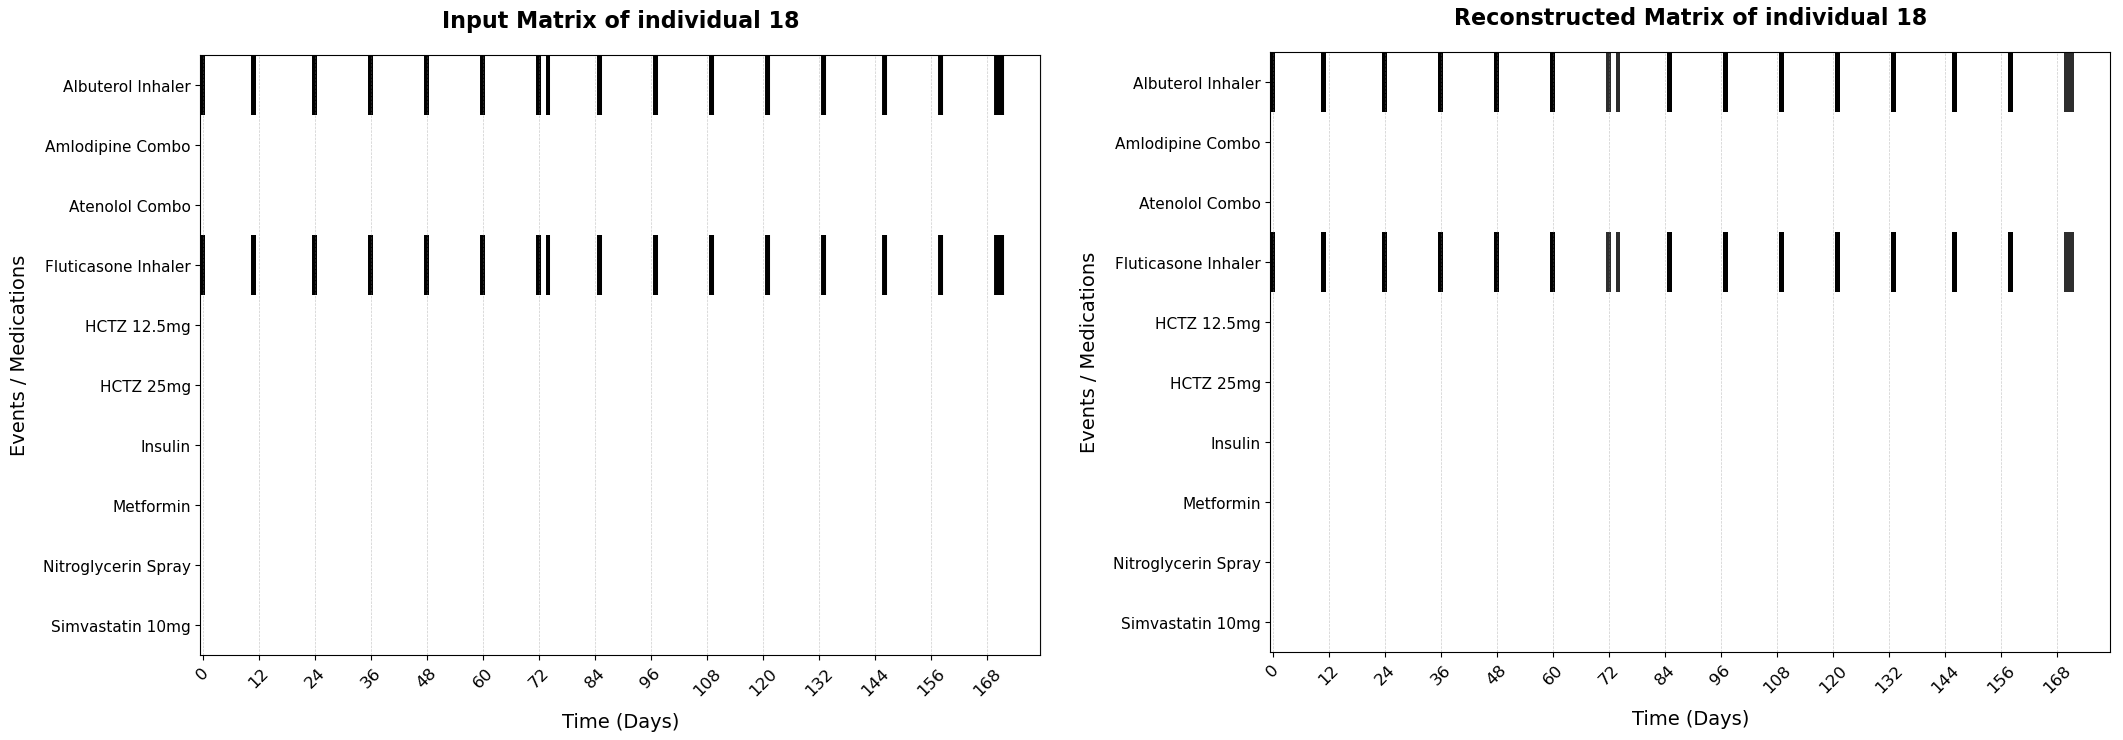
\includegraphics[width=\textwidth]{rec_pat18_SYNTHEA.png}
    \caption{Input matrix (left) and reconstructed matrix (right) for patient~18 in the Synthea cohort.}
    \label{fig:rec18_synthea}
\end{figure}

\begin{figure}[htbp]
    \centering
    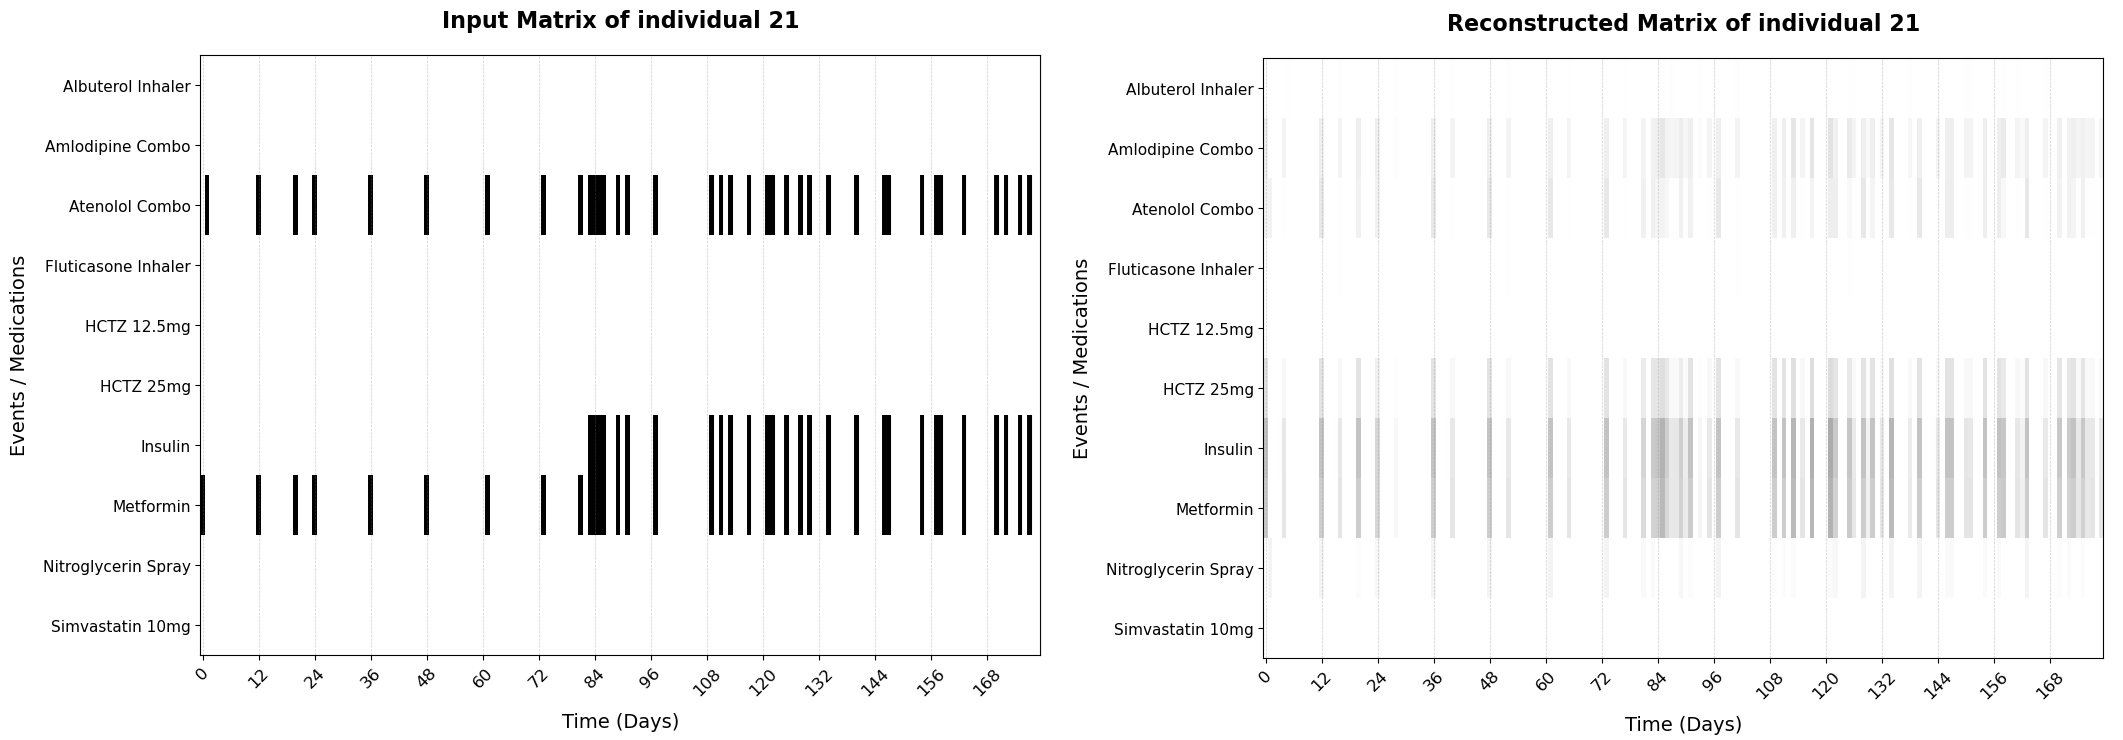
\includegraphics[width=\textwidth]{rec_pat21_SYNTHEA.png}
    \caption{Input matrix (left) and reconstructed matrix (right) for patient~21 in the Synthea cohort.}
    \label{fig:rec21_synthea}
\end{figure}

\begin{figure}[htbp]
    \centering
    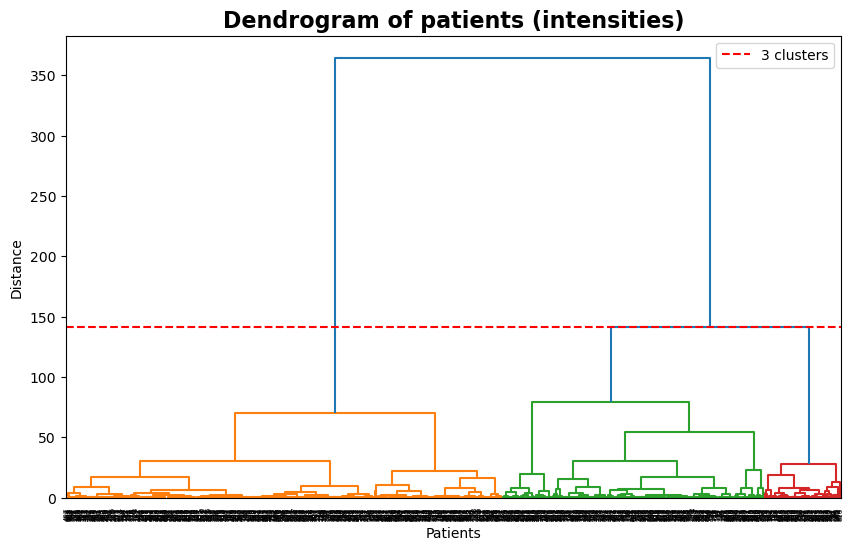
\includegraphics[width=\textwidth]{dendrogramme_SYNTHEA.png}
    \caption{Dendrogram of the 901 Synthea patients obtained by hierarchical agglomerative clustering (Ward linkage, Euclidean distance) applied to the normalised phenotype intensity vectors.}
    \label{fig:dendro_synthea}
\end{figure}

\begin{figure}[htbp]
    \centering
    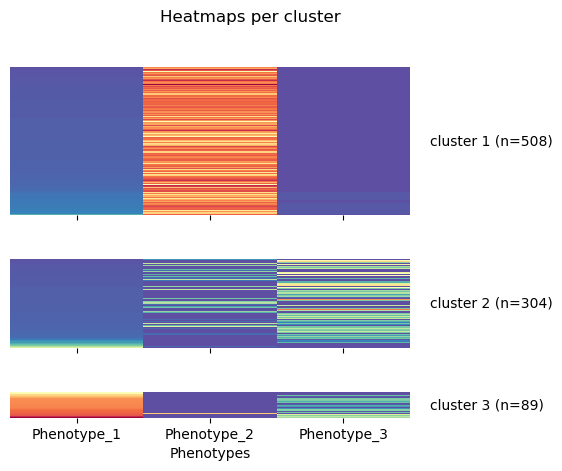
\includegraphics[width=0.85\textwidth]{heatmap_SYNTHEA.png}
    \caption{Per-cluster heatmaps of normalised phenotype intensities for the three patient clusters identified in the Synthea cohort. 
    Each row represents a patient, each column a phenotype, and the colour encodes the intensity of phenotype activation, ranging from low (dark blue) to high (dark red).}
    \label{fig:heatmap_synthea}
\end{figure}

\FloatBarrier

\subsubsection{VICAN5 real cohort}\label{sec:vican_res}

\textbf{Experimental setup.}
The tensor constructed from the VICAN5 dataset has dimensions $K = 1 336$ patients, $n = 4$ event types, and a maximum follow-up duration of $\bar{T} = 24$ months. 
Training settings match Synthea: up to 500 epochs, early stopping with patience of 5 epochs monitored on $\text{FIT}_X$, learning rate $10^{-2}$, and a \emph{ReduceLROnPlateau} scheduler.

\textbf{Hyperparameter search.}
A random search over 10 configurations was performed with \texttt{random.seed(42)}, drawing configurations uniformly (both regularisation weights on a log scale) from: rank $R \in \{2, \ldots, 4\}$, window length $\omega \in \{2, \ldots, 5\}$ months, normalised sparsity weight $\tilde{\alpha} \in [10^{-5},\, 10^{-3}]$, normalised non-succession weight $\tilde{\gamma} \in [0.1,\, 10.0]$. 
The rank was bounded above by the number of treatment modalities ($n = 4$), and the window length upper bound reflects the typical duration of a treatment episode in colorectal cancer care. 
The total search required approximately 29 hours of computation.

\textbf{Results.}
The configuration retained for interpretation ranked sixth by $\text{FIT}_X$ but was selected for phenotypic interpretability: rank $R = 3$, window length $\omega = 3$ months, normalised weights $\tilde{\alpha} = 0.28$ and $\tilde{\gamma} = 0.36$ ($\alpha = 7.91 \times 10^{-5}$, $\gamma = 0.36$).
 
Over 110 epochs (Figure~\ref{fig:training_vican5}), the total loss decreases from almost 9000 to around 1000 at convergence, while $\text{FIT}_X$ increases from 0.02 to a peak of 0.52 around epoch~60 before declining as the non-succession term begins to dominate, reaching a final $\text{FIT}_X = 0.51$. 
The retained configuration achieves a phenotypic diversity $\text{div}(\mathcal{P}) = 1.0$, confirming that the three phenotypes are well separated.
 
The three discovered phenotypes (Figure~\ref{fig:phenos_vican5}) are clinically interpretable: 
\begin{itemize}
  \item \textbf{Phenotype~1} captures moderate simultaneous oral chemotherapy and radiotherapy activation concentrated at month~0; 
  \item \textbf{Phenotype~2} shows strong, sustained intravenous chemotherapy activation over the full $\omega = 2$-month window.
  \item \textbf{Phenotype~3} corresponds to moderate surgical activation at month~0; 
\end{itemize}

Reconstruction of individual trajectories was overall satisfactory. 
For patient~8 (Figure~\ref{fig:rec_vican5}), the reconstructed matrix faithfully recovers the dominant temporal structure, correctly localising the IV chemotherapy period (months~3-10) and early treatment events at month~0, with activations somewhat attenuated relative to the binary input but the overall pattern well preserved.

\textbf{Clustering.}
A pairwise Euclidean distance matrix on the normalised phenotype intensity vectors, followed by HAC (Ward linkage), revealed a clear four-cluster structure (Figure~\ref{fig:dendro_vican5}) with different types of patients in these clusters (Figure~\ref{fig:heatmap_vican5}): 
\begin{itemize}
  \item Cluster~1 ($n_1 = 212$) shows very strong Phenotype~2 (IV chemotherapy) showing a cluster of patients only receiving IV chemotherapy, with very weak activations of Phenotypes~1 and~3 (oral chemotherapy, radiotherapy, and surgery); 
  \item Cluster~2 ($n_2 = 551$) shows a moderate activation of Phenotype~2 (IV chemotherapy) with weak activations of Phenotype~3 (surgery) and even weaker activation of Phenotype~1 (oral chemotherapy and radiotherapy); 
  \item Cluster~3 ($n_3 = 371$) shows Phenotype~3 (surgery), containing the patients that only had to have surgery in their treatments;
  \item Cluster~4 ($n_4 = 202$) shows low activation of Phenotype~1 (oral chemotherapy and radiotherapy).
\end{itemize}


\begin{figure}[htbp]
    \centering
    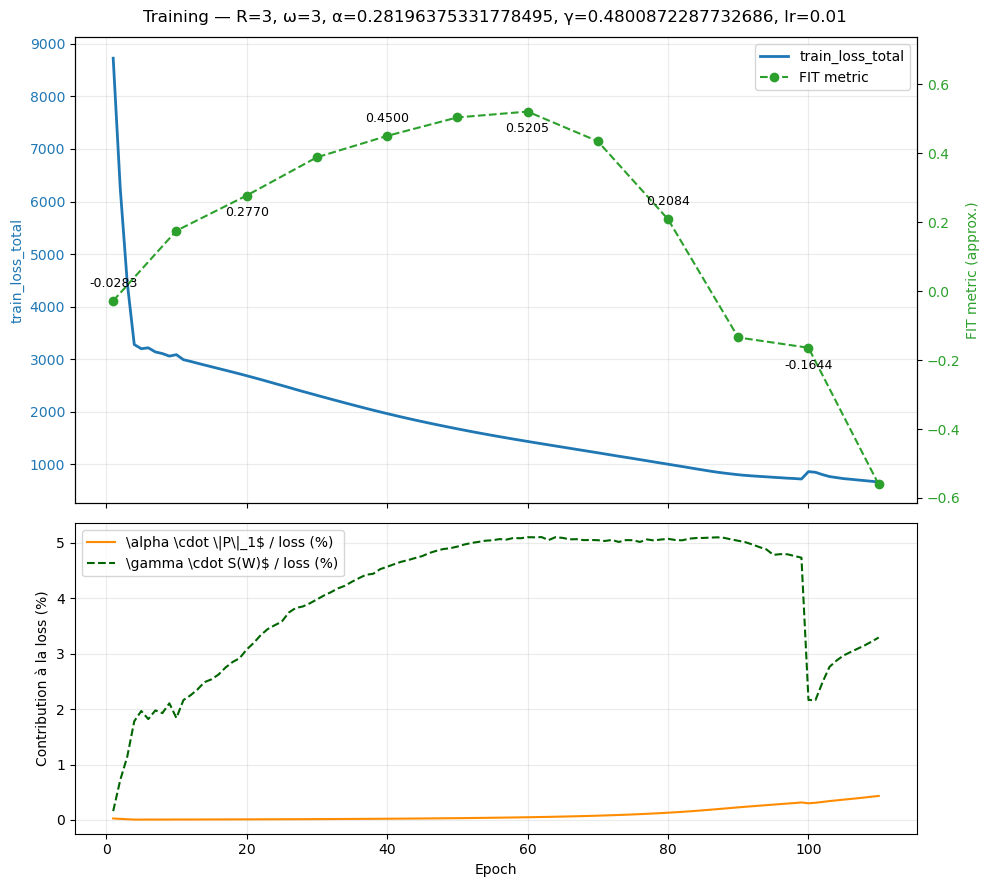
\includegraphics[width=\textwidth]{training_VICAN.png}
    \caption{Training history of the retained SWoTTeD configuration on the VICAN5 cohort ($R=3$, $\omega=3$, $\tilde{\alpha}=0.282$, $\tilde{\gamma}=0.480$, $\text{lr}=10^{-2}$). 
    \textit{Top}: total training loss (blue) and approximate $\text{FIT}_X$ metric (green dashed) over 110 epochs. 
    \textit{Bottom}: relative contributions of the sparsity term $\alpha\cdot\|\mathcal{P}\|_1$ (orange) and the non-succession term $\gamma\cdot S(\mathcal{W})$ (green dashed) to the total loss.}
    \label{fig:training_vican5}
\end{figure}

\begin{figure}[htbp]
    \centering
    
\includegraphics[width=\textwidth]{phenos_VICAN.png}
    \caption{The three phenotypes discovered by SWoTTeD on the VICAN5 cohort ($R=3$, $\omega=3$, $\tilde{\alpha}=0.282$, $\tilde{\gamma}=0.480$, $\text{lr}=10^{-2}$).}
    \label{fig:phenos_vican5}
\end{figure}

\begin{figure}[htbp]
    \centering
    
\includegraphics[width=\textwidth]{rec_pat8_VICAN.png}
    \caption{Input matrix (left) and reconstructed matrix (right) for patient~8 in the VICAN5 cohort.}
    \label{fig:rec_vican5}
\end{figure}

\begin{figure}[htbp]
    \centering
    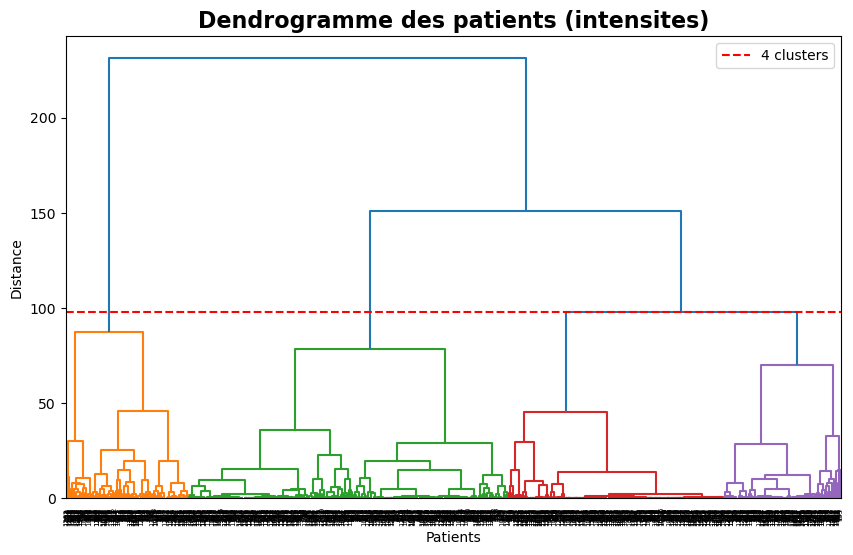
\includegraphics[width=\textwidth]{dendrogramme_VICAN.png}
    \caption{Dendrogram of the 1,336 VICAN5 patients obtained by hierarchical agglomerative clustering (Ward linkage, Euclidean distance) applied to the normalised phenotype intensity vectors. 
    The red dashed line indicates the cut corresponding to four clusters.}
    \label{fig:dendro_vican5}
\end{figure}

\begin{figure}[htbp]
    \centering
    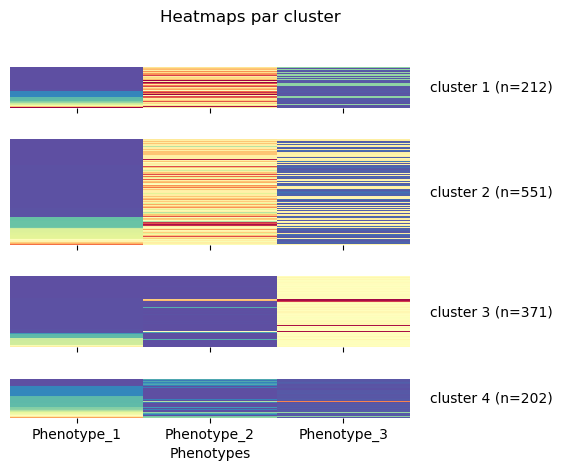
\includegraphics[width=0.85\textwidth]{heatmap_VICAN.png}
    \caption{Per-cluster heatmaps of normalised phenotype intensities for the three patient clusters identified in the VICAN5 cohort ($n_1=212$, $n_2=551$, $n_3=371$, $n_4=202$).
    Each row represents a patient, each column a phenotype, and the colour encodes the intensity of phenotype activation, ranging from low (dark blue) to high (dark red).}
    \label{fig:heatmap_vican5}
\end{figure}

\FloatBarrier

\section{Discussion}\label{sec:discussion}

\subsection{Unidimensional analysis}\label{sec:disc_uni}

\pkg{TCA} reproduced the four-cluster structure obtained with \pkg{TraMineR} on the same dataset, with clinically interpretable profiles: \textit{Fast}, \textit{Slow}, \textit{Incomplete}, and \textit{Out of care} correspond to distinct progression patterns through the care continuum, from persistent disengagement to rapid progression toward controlled infection.
 
A limitation of the unidimensional module is computation time: while most metrics are fast, DTW takes approximately 4~minutes and GAK approximately 6~minutes on this dataset, due to the quadratic complexity of pairwise distance computation, which may take longer for larger cohorts.
 
\pkg{TraMineR}, implemented in \proglang{R}, primarily supports unidimensional representations; \pkg{TCA} is, to our knowledge, the first \proglang{Python} package offering a unified framework for both unidimensional and multidimensional care trajectory analysis.

\subsection{Multidimensional analysis}\label{sec:disc_multi}

\textbf{Computational cost.}
The SWoTTeD decomposition is computationally demanding, as each training run involves iterative gradient-based optimisation over a high-dimensional tensor. 
Table~\ref{tab:compute_vican5} reports computation times and parameters for the shortest and longest training runs on the VICAN5 cohort across the 10 random search configurations. 

\begin{table}[htbp]
\centering
\caption{Computation times and model characteristics for the shortest and longest training runs on the VICAN5 cohort ($K=1 336$ patients, $n=4$ event types, $\bar{T}=24$ months).}
\label{tab:compute_vican5}
\begin{tabular}{lcccccc}
\toprule
 & $R$ & $\omega$ & $\tilde{\alpha}$ & $\tilde{\gamma}$ & Time \\
\midrule
Shortest & $4$ & $3$ & $0.723$ & $2.527$ & $3 195$~s \\
Longest  & $2$ & $5$ & $0.050$ & $9.909$ & $7 555$~s \\
\bottomrule
\end{tabular}
\end{table}

\textbf{Balancing reconstruction quality, diversity, and interpretability.}
A central challenge in applying SWoTTeD to real-world data is finding a configuration achieving satisfactory reconstruction quality, diverse phenotypes, and clinical interpretability at once. 
These objectives are not always aligned: high $\text{FIT}_X$ may yield phenotypes too similar to be clinically distinguished, while high diversity may cost reconstruction quality. 
Visually interpretable phenotypes do not always match the best numerical scores, as shown by VICAN5, where the retained configuration ranked sixth by $\text{FIT}_X$ yet was the most clinically coherent.
 
On Synthea, $\text{FIT}_X$ reached $0.576$, consistent with the controlled nature of synthetic data. 
On VICAN5, retained configurations reached $0.58$, lower than the $\sim\!0.7$ reported by \cite{sebia2024swotted} on other datasets, likely reflecting the greater heterogeneity and sparsity of real-world clinical trajectories.
 
To navigate this trade-off, \pkg{TCA} implements complementary strategies: early stopping on $\text{FIT}_X$ limits optimisation once reconstruction plateaus; a \emph{ReduceLROnPlateau} scheduler helps stabilise training; and a diversity metric $\text{div}(\mathcal{P})$ is tracked alongside $\text{FIT}_X$ during random search. 
These criteria are necessary but not sufficient: visual inspection remains essential, since similar numerical scores can yield very different interpretability. 
This points to a broader consideration: automated hyperparameter optimisation cannot fully replace domain knowledge, and integrating clinical expertise into model selection remains important for meaningful, interpretable phenotypes.

\section{Conclusion}\label{sec:conclusion}

This study presented \pkg{TCA} (Trajectory Clustering Analysis), an open-source \proglang{Python} package providing a unified framework for analyzing longitudinal care trajectories in both unidimensional and multidimensional settings.
 
The unidimensional module integrates multiple dissimilarity measures and clustering algorithms, and recovered clinically interpretable trajectory profiles on a real-world clinical sequence dataset. The multidimensional module integrates SWoTTeD~\cite{sebia2024swotted}, extending the analysis to settings where multiple care events may co-occur; applied to a synthetic cohort and a real-world colorectal cancer cohort, it identified distinct temporal phenotypes and supported clinically interpretable patient typologies.
 
These experiments also highlighted a practical challenge: reconstruction quality, phenotypic diversity, and clinical interpretability are not necessarily aligned, so hyperparameter selection cannot rely on a single criterion and visual inspection remains important. Future work will focus on more data-adaptive hyperparameter selection strategies, reducing computational cost and subjectivity.
 
More broadly, \pkg{TCA} is not restricted to oncology and can be applied to any longitudinal biomedical dataset in which clinical or healthcare events are recorded over time, bringing unidimensional trajectory clustering and multidimensional temporal tensor decomposition into a single \proglang{Python} framework to facilitate advanced trajectory analysis in biomedical research.

\section*{Availability and requirements}
\begin{itemize}
  \item \textbf{Project name:} TCA (Trajectory Clustering Analysis)
  \item \textbf{Project home page:}
        \url{https://github.com/QuanTIMLab/TrajectoryClusteringAnalysis}
  \item \textbf{Operating system:} Platform independent
  \item \textbf{Programming language:} \proglang{Python} $\geq 3.6$
  \item \textbf{Other requirements:} \proglang{PyTorch}, \proglang{PyTorch Lightning}
  \item \textbf{License:} MIT
\end{itemize}

\section*{Ethics approval and consent to participate}
The Synthea \citep{walonoski2020synthea} dataset is fully synthetic and contains no real human data.
The \textit{unidimensional\_data} dataset is an open-access educational dataset provided by Larmarange \citep{larmarange_analyseR} for statistical training purposes. It is distributed for methodological demonstration without identifiable personal data.
The VICAN5 \citep{Bouhnike005971} dataset was collected as part of a national survey whose methodology was approved by three national ethics commissions: 
the CCTIRS (Comité Consultatif sur le Traitement de l’Information en Matière de Recherche dans le Domaine de la Santé, study registered under no 11-143), 
the ISP (Institute of Public Health, study registered under no C11-63) 
and the CNIL (French Commission on Individual Data Protection and Public Liberties, study registered under no 911290). 
Confidentiality is assured for all participants with regard to any personal responses and information provided, as all data collected are anonymised.

\section*{Consent for publication}
Not applicable.

\section*{Availability of data and materials}
The datasets used and analyzed during the current study are available at \url{https://github.com/QuanTIMLab/TrajectoryClusteringAnalysis}.

\section*{Competing interests}
The authors declare that they have no competing interests.

\section*{Funding}
A REMPLIR

\section*{Acknowledgements}
A REMPLIR

\bibliographystyle{elsarticle-num}
\bibliography{cas-refs}

\printcredits

\end{document}